% Winter Geometry Workshop 2026 — poster (Christmas version)
% Needs CalabiYau-christmas.png in the same folder.
% Compile with: pdflatex WinG-Poster.tex
\documentclass[a4paper,12pt]{article}

\usepackage[margin=18mm,top=16mm,bottom=14mm]{geometry}
\usepackage[T1]{fontenc}
\usepackage[utf8]{inputenc}
\usepackage{charter}
\usepackage{microtype}
\usepackage{xcolor}
\usepackage{graphicx}
\usepackage{hyperref}

\definecolor{ink}{HTML}{16232E}
\definecolor{holly}{HTML}{A81F2D}
\definecolor{pine}{HTML}{12633C}
\definecolor{palepine}{HTML}{C8DACF}

\hypersetup{colorlinks=true, urlcolor=pine, pdftitle={Winter Geometry Workshop 2026},
            pdfauthor={Pietro Mesquita-Piccione}}

\pagestyle{empty}
\color{ink}
\setlength{\parindent}{0pt}

\begin{document}

{\color{palepine}\rule{\linewidth}{1.2pt}}

\vspace{6mm}

{\fontsize{13}{16}\selectfont University of Gothenburg and Chalmers University of Technology}

\vspace{9mm}

{\fontsize{40}{46}\selectfont\bfseries Winter Geometry\\[2mm] Workshop}

\vspace{7mm}

{\fontsize{20}{24}\selectfont\color{holly} 9--11 December 2026}

\vspace{4mm}

{\fontsize{13}{17}\selectfont Department of Mathematical Sciences, Chalmers Tvärgata 3, Gothenburg}

\vfill

\begin{minipage}[t]{0.52\linewidth}
  \vspace{0pt}\raggedright
  {\fontsize{13}{18}\selectfont The talks will cover complex geometry, including pluripotential theory, canonical metrics and K-stability, and connections with mathematical physics.}

  \vspace{9mm}

  {\fontsize{16}{19}\selectfont\bfseries Speakers}

  \vspace{3mm}

  {\fontsize{13}{21}\selectfont
  %Robert Berman \textit{(TBC)}\\
  Bo Berndtsson\\
  Sébastien Boucksom\\
  Yifan Chen\\
  Ruadhaí Dervan \\
  Siarhei Finski\\
  Henri Guenancia\\
  Hans-Joachim Hein\\
  Semyon Klevtsov\\
  Chi Li\\
  Zakarias Sjöström Dyrefelt\par}
\end{minipage}\hfill
\begin{minipage}[t]{0.5\linewidth}
  \vspace{50pt}
  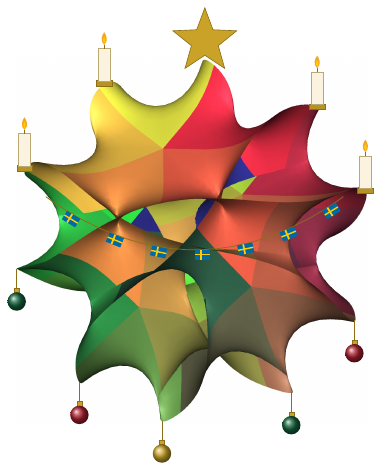
\includegraphics[width=0.9\linewidth]{deco-tree.png}
\end{minipage}

\vfill

{\color{palepine}\rule{\linewidth}{0.6pt}}

\vspace{4mm}

{\fontsize{12.5}{17}\selectfont
Registration is free and open until 9 November 2026 at \texttt{pietropic.github.io/wing-workshop}.\\
Organized by Pietro Mesquita Piccione. Questions to \texttt{piccione@chalmers.se}.\\[2mm]
{\color{pine}Supported by Wilhelm och Martina Lundgrens Vetenskapsfond.}}

\end{document}
